\documentclass[zavrsnirad]{fer}
% Dodaj opciju upload za generiranje konačne verzije koja se učitava na FERWeb
% Add the option upload to generate the final version which is uploaded to FERWeb


\usepackage{blindtext}
\usepackage{tabularray}
\usepackage{xltabular} % for xltabular environment
\usepackage{amsmath} % for mathematical symbols and formatting
\usepackage{graphicx} % Include the graphicx package


%--- PODACI O RADU / THESIS INFORMATION ----------------------------------------

% Naslov na engleskom jeziku / Title in English
\title{Intelligent player for Prisoner's Dilemma}

% Naslov na hrvatskom jeziku / Title in Croatian
\naslov{Inteligentni igrač za Zatvorenikovu dilemu}

% Broj rada / Thesis number
\brojrada{1678}

% Autor / Author
\author{Petar Belošević}

% Mentor 
\mentor{Prof. Marko Čupić}

% Datum rada na engleskom jeziku / Date in English
\date{June, 2024}

% Datum rada na hrvatskom jeziku / Date in Croatian
\datum{lipanj, 2024.}

%-------------------------------------------------------------------------------


\begin{document}


% Naslovnica se automatski generira / Titlepage is automatically generated
\maketitle


%--- ZADATAK / THESIS ASSIGNMENT -----------------------------------------------

% Zadatak se ubacuje iz vanjske datoteke / Thesis assignment is included from external file
% Upiši ime PDF datoteke preuzete s FERWeb-a / Enter the filename of the PDF downloaded from FERWeb
\zadatak{Extra/hr-0036538383-73.pdf}


%--- ZAHVALE / ACKNOWLEDGMENT --------------------------------------------------

\begin{zahvale}
  % Ovdje upišite zahvale / Write in the acknowledgment
\end{zahvale}


% Odovud započinje numeriranje stranica / Page numbering starts from here
\mainmatter


% Sadržaj se automatski generira / Table of contents is automatically generated
\tableofcontents


%--- UVOD / INTRODUCTION -------------------------------------------------------
\chapter{Uvod}
\label{pog:uvod}

Neki od radova koje ćemo citirati su \cite{6248073,6247753,ghiglia_pritt_phase_unwrapping,hartley2003multiple,4250461,123DCatch}.
Trebaju nam samo radi testiranja kako izgleda referenciranje rada s konferencije, rada iz časopisa, knjige i Internetske stranice.

\begin{figure}[htb]
  \centering
  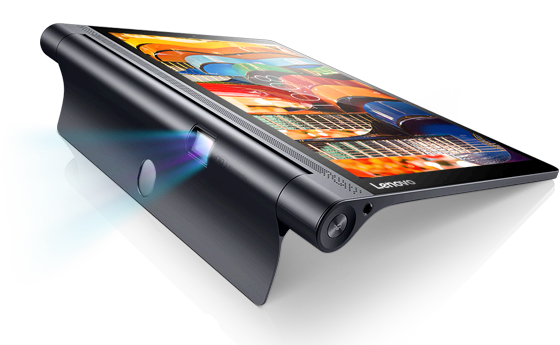
\includegraphics[width=0.38\linewidth]{Extra/lenovo_yoga_tab3_pro_front.png} 
  \caption{Moja prva slika}
  \label{slk:prvaslika}
\end{figure}

Referenciramo se na sliku \ref{slk:prvaslika} u sredini rečenice, zatim prije zareza \ref{slk:prvaslika}, te zatim na kraju rečenice \ref{slk:prvaslika}.
Upravo smo testirali radi li naredba \verb|\ref| ispravno u slučaju kada nakon nje slijedi točka.

Sada slijedi jedna jednadžba:
\begin{equation}
  \label{jed:prvajednadzba}
  \int_{-\infty}^{+\infty}f(t)\,dt=F(\omega)
\end{equation}
Jednadžba \eqref{jed:prvajednadzba} je moja prva jednadžba koja definira par $f(t)\ufrek F(\omega)$ ili $F(\omega)\uvrem f(t)$.

\cite{1980Axelrod1}
\cite{1980Axelrod2}
\cite{igraHrEnc}

\break

	Zatvorenikova dilema jedan je od najpoznatijih problema iz područja teorije igara. Dilema proučava interakciju između dvaju pojedinaca kroz igru suradnje i izdaje. Zatvorenikova dilema se može pronaći u korijenu mnogih interakcija koje se pojavljuju u društvu, ali i u životinjskom svijetu. Glavno pitanje je kako ta interakcija utječe na dobrobit oba igrača. Paradoks u Zatvorenikove dileme je činjenica da racionalno razmišljanje navodi svakog pojedinca da odabire opciju koja ne odgovara niti jednom od igrača \cite{PrisDilemmaHrEnc}.
	
	U stvarnom životu su takve interakcije često ponavljajuće prirode. Tada je potrebno imati na umu da će druga strana vjerojatno imati iskustvo prošlih interakcija što može utjecati na njihovu odluku u novoj interakciji. Stoga je interesantno razmatranje malo složenijeg problema iterirajuće Zatvorenikove dileme. Zanimljivo je da se u iterirajućem problemu mijenja pristup optimalnoj strategiji u odnosu na jednokratnu Zatvorenikovu dilemu.
	
	U korijenu Zatvorenikove dileme je napetost između individualnog racionalizma (u pogledu da je objema stranama smisleno biti sebičan) i grupnog racionalizma (objema stranama je isplativija obostrana suradnja nego obostrana izdaja) \cite{1980Axelrod1}.
	
	Mnogo je radova na pisano na temu optimalnog načina igranja Zatvorenikove dileme. Tako je Robert Axelrod iz Sveučilišta u Michiganu održao dva turnira u kojima su sudionici predavali svoje strategije za igranje igre u obliku računalnih programa \cite{1980Axelrod1} \cite{1980Axelrod2}. Analizom turnira došlo se zanimljivih zaključaka. Axelrod je proučavanjem strategija i njihovih rezultata izlučio nekoliko karakteristika koje imale tendenciju davati bolje rezultate. Te karakteristike su ljubaznost, opraštanje i provokabilnost \cite{1980Axelrod2}.
	
	Glavni cilj ovog rada je napraviti model inteligentnog igrača koji će naučiti igrati iterirajuću Zatvorenikovu dilemu. Cilj ovoga je proučiti kakvo će ponašanje razviti inteligentni igrač i kako će igrati protiv nekih drugih poznatih strategija. Također će biti zanimljivo analizirati ponašanje inteligentnog igrača i vidjeti je li razvio karakteristike koje su se pokazale poželjnima u Axelrodovim turnirima.

%-------------------------------------------------------------------------------
\chapter{Zatvorenikova dilema}
\label{pog:ZatvorenikovaDilema}

	Zatvorenikova dilema je poznati problem iz područja teorije igara koji proučava odnose između pojedinaca. Radi se o igri sa dva igrača koji imaju na izboru dva poteza: suradnja sa drugim igračem ili izdaja drugog igrača. S obzirom na odabir oba igrača, svakom od njih se daje određena kazna ili nagrada. 
	
	Dilema je dobila naziv po ilustrativnom opisu Alberta Tuckera \cite{TeorijaIgaraIPravo}. Dilema je opisana u kontekstu odvojenog ispitivanja dvojice osumnjičenih kriminalaca. Svaki od osumnjičenih može priznati krivnju (ekvivalentno izdaji) ili šutjeti (ekvivalentno suradnji). Sukladno njihovim potezima dodjeljuju im se zatvorske kazne. Ako i jedan i drugi osumnjičenik šute, dobivanju male zatvorske kazne zbog nedostatka dokaza. Ako i jedan i drugi priznaju krivnju, svatko od njih dobiva veće zatvorske kazne jer su priznali krivnju. Ako pak jedan od njih prizna krivnju a drugi šuti, ovaj koji je priznao krivnju biva oslobođen optužbi kao nagrada za suradnju, a drugi dobiva još veću zatvorsku kaznu zbog toga što je odugovlačio postupak odbijanjem priznavanja krivice \cite{TeorijaIgaraIPravo}.
	
	Dilema se naravno može staviti i opisati kroz razne slikovite kontekste. No, u ovom radu će se radi jednostavnosti na dilemu gledati samo kao igru u kojoj igrači skupljaju bodove.

	Generalna pravila za "bodovanje" je da obostrana suradnja i obostrana izdaja daju simetričnu podjelu bodova, uz to da suradnja daje veći broj bodova. U slučaju da jedan igrač surađuje dok ga drugi izdaje dolazi do nesimetrične podjele bodova. Igrač koje je izdan mora dobiti manje bodove nego bi dobio obostranom izdajom. Igrač koji ga je izdao tim potezom mora dobiti više nego bi dobio obostranom suradnjom. Tipična raspodjela bodova \cite{1980Axelrod1} koja će se koristiti i u ovom radu dana je u tablici \ref{Payoffs}.
	 
	Važno je primijetiti da je Zatvorenikova dilema igra s promjenjivim ishodom \cite{PrisDilemmaHrEnc}. To znači da dobitak jednog igrača nije nužno gubitak drugog igrača i gubitak jednog igrača ne mora nužno biti dobitak drugog igrača \cite{igraHrEnc}. Drugim riječima, mogući su ishodi u kojima oba igrača profitiraju ili oba igrača gube. Upravo ova karakteristika omogućuje suradnji da bude poželjan pristup igranju. 
	
	\begin{longtblr}[
		caption={Bodovanje odluka igrača u Zatvorenikovoj dilemi \\
			Napomena: Bodovi Igrača 1 su dani prvim brojem u svakom od parova.},
		label=Payoffs,
		entry=none
		]{
			width = \textwidth,
			colspec={|X[1,l]|X[2, l]|X[2, l]|X[2,l]|}, 
			rowhead = 0,
		} %definicija širine tablice, širine stupaca, poravnanje i broja redaka naslova tablice
		\hline 
		\SetCell[c=2, r=2]{c,r}{} & & \SetCell[c=2]{c}{Igrač 2} \\ \hline
		& & Suradnja & Izdaja \\ \hline
		\SetCell[r=2]{r}{Igrač 1} & Suradnja & 3, 3 & 0, 5 \\ \hline
		& Izdaja & 5, 0 & 1, 1 \\ \hline
	\end{longtblr}
	 
	Zbog ove karakteristike Zatvorenikova dilema dobro opisuje mnoge probleme iz stvarnog života i objašnjava zašto je ponekad suradnja sa neprijateljem poželjna. Poznati je takav primjer problem prekomjernog naoružavanja i međusobnog nepovjerenja SAD-a i SSSR-a tijekom hladnog rata \cite{1980Axelrod1} Upravo je i taj problem bio jedan od motiva nastanka i proučavanja Zatvorenikove dileme.
	
	Zatvorenikova dilema dobro modelira određena ponašanja nekih životinjskih vrsta u prirodi. Tako je primijećeno ponašanje nazvano \textit{inspekcija predatora} kod nekih vrsta riba kao što su gupi riba (lat. \textit{Poecilia reticulata}) i koljuška (lat. \textit{Gasterosteus aculeatus}). \cite{TheEvolutionOfCooperation}
	
	Također je primijećena međusobna suradnja kod imapla koje se međusobno timare kako bi se štitile od krpelja. No, zbog nedostatka informacija o cijeni i nagradi za ovakvo ponašanja teško je ovaj primjer modelirati Zatvorenikovom dilemom. \cite{TheEvolutionOfCooperation}

	\section{Dobra strategija}
	\label{pog:DobraStrategija}
	
		Pitanje koje se prirodno nameće u Zatvorenikovoj dilemi je dosta očito: Kako dobro igrati ovu igru? Kojom strategijom pristupiti ovoj igri?

		U svrhu istraživanja optimalnih strategija Robert Axelrod je 1980. organizirao turnir \cite{1980Axelrod1} u koji je pozvao znanstvenike iz raznih područja koji su se bavili Zatvorenikovom dilemom. Učesnici su za turnir izradili strategije igranja Zatvorenikove dileme u obliku računalnog programa. Svaka strategija je igrala Zatvorenikovu dilemu u 200 iteracija sa svakom drugom strategijom, sa samom sobom i sa dodatnom strategijom koja je donosila nasumične odluke. Kasnije te godine Axelrod je organizirao još jedan sličan turnir u svrhu provođenja dodatne analize \cite{1980Axelrod2}.
	
		Pobjednik u oba turnira je bila strategija zvana \textit{Tit for Tat}, također poznata i kao \textit{Copycat}. Strategija je vrlo jednostavna - na prvom potezu uvijek surađuje, a dalje uvijek kopira suparnikov prethodni potez \cite{1980Axelrod1}.
	
		Axelrod je analizom rezultata oba turnira pronašao nekoliko karakteristika koje su bile ključne za uspješnost strategija u oba turnira. Pronađene karakteristike su:
		\begin{itemize}
			\item \textbf{Ljubaznost} (eng. \textit{niceness}) \cite{1980Axelrod1} - strategija je ljubazna ako nikada neće prva izdati drugog igrača
			\item \textbf{Sklonost opraštanju} (eng. \textit{forgiveness}) \cite{1980Axelrod1} - sklonost strategije da surađuje nakon što ju je drugi igrač izdao
			\item \textbf{Provokabilnost} (eng. \textit{provocability}) \cite{1980Axelrod2} - sklonost da strategija izda drugog igrača nakon što ju je drugi igrač izdao
		\end{itemize}
		
		Valja primijetiti da su karakteristike sklonosti opraštanju i provokabilnost zapravo u suprotnosti. No one nisu binarne (ili su prisutne u strategiji ili nisu) neko se pojavljuju u strategijama u nekoj mjeri. Zbog toga nisu međusobno isključive.
	
		Strategija \textit{Tit for Tat} je bila uspješna jer je bila ljubazna te je imala dobru ravnotežu između sklonosti opraštanju i provokabilnosti. \textit{Tit for Tat} je ljubazna strategija jer počinje sa suradnjom i izdaje samo ako ju je drugi igrač izdao prvi. Strategija oprašta jer će nakon što bude jedom izdana uzvratiti izdajom, ali će nakon toga nastaviti surađivati dok ponovno ne bude izdana - strategija pamti samo prijašnji potez suparnika. Također, strategija je provokabilna jer će nakon što bude izdana uvijek uzvratiti izdajom.
		
		Valja zamijetiti jednu vrlo zanimljivu činjenicu. Ako malo razmislimo o strategiji \textit{Tit for Tat}, možemo primijetiti da ta strategija nikada ne može igrati bolje od igrača sa kojim igra Zatvorenikovu dilemu. U najboljem slučaju strategija \textit{Tit for Tat} može dobiti jednak broj bodova kao i drugi igrač. Ovo pokazuje da kod iterirajuće zatvorenikove dileme nije uvijek nužno biti bolji od drugog igrača, već igrati kontinuirano dobro sa različitim strategijama. 
	
		Axelrod je u svojem radu napomenuo važnu stvar, a to je da ne postoji najbolja strategija za Zatvorenikovu dilemu. To proizlazi iz jednostavne činjenice da performansa strategije uvelike ovisi o strategijama s kojima ta strategija igra. Dakle, okruženje u kojem se nalazi je od presudne važnosti \cite{1980Axelrod1}.
	
		No kroz detaljnu analizu drugog turnira Axelrod je ustanovio da su navedene karakteristike generalno poželjne i u pravilu donose dobre rezultate. Također, iako \textit{Tit for Tat} nije univerzalno najbolja strategija, pokazuje se da generalno daje odlične rezultate u raznim okruženjima zbog dobro kombiniranih poželjnih karakteristika \cite{1980Axelrod2}.
	
		Axelrod je također napomenuo da je kod kreiranja strategije potrebna analiza na barem 3 dubine \cite{1980Axelrod1}. Prva razina je direktna posljedica trenutne odluke, to jest, koliko bodova igrač dobiva na temelju svoje odluke. Druga razina je uzimanje u obzira da će drugi igrač možda odlučiti kazniti izdaju. Treća razina razmatra da reagiranje na izdaju može prouzrokovati eho efekt međusobnih izdaja koji će dugoročno štetiti i jednom i drugom igraču.

\chapter{Umjetne neuronske mreže}
\label{pog:NeuronskeMreze}
	
	Umjetne neuronske mreže su jedan od mnogih koncepata u strojnom učenju, koje je jedno od najvećih grana umjetne inteligencije. Prvi puta su ih predložili Warren McCullough i Walter Pitts sa Sveučilišta u Chicagu davne 1944. Prva neuronska mreža koja se mogla trenirati je bila Perceptron, a predložio ju je psiholog Frank Rosenblatt sa Sveučilišta Cornell 1957. \cite{MITNeuralNet}
	
	Umjetne neuronske mreže su inspirirane ljudskim mozgom - sastoje se od velikog broja jednostavnih umjetnih neurona koji su gusto povezani. \cite{MITNeuralNet}
	
	Područje koje se bavi umjetnim neuronskim mrežama zove se neuro-računarstvo, koje čini granu računarstva iz skupine mekog-računarstva. Meko računarstvo objedinjuje pristupe čiji je cilj izgraditi tehničke sustave za rješavanje teških problema sa čestim šumom i nepouzdanošću u ulaznim podacima. \cite{skriptaNeuronskeMreze} 
	
	Umjetni neuron je najmanja funkcionalna jedinka neuronske mreže i modelira biološki neuron u ljudskom mozgu. Umjetni neuroni imaju ulogu jednostavne procesne jedinice. Svaki umjetni neuron na ulazu prima nekakve numeričke vrijednosti (izlazi drugih neurona ili ulazni podaci), obično označene kao vektor $\vec{x}$. Svaki ulazni podatak u neuron $x_i$ se prvo množe sa težinom veze $w_i$ preko koje je došao do trenutnog neurona. Dobiveni umnošci se zbrajaju, te im se dodatno pribraja takozvani pomak (eng. \textit{bias}), obično označavan sa $w_0$. Tako nastala suma se obično označava sa \text{net} te se može izraziti formulom \ref{net}. Ako se pak vektor ulaznih podataka umjetno proširi sa komponentom $x_0$ koja ima fiksnu vrijednost $1$, onda se formula za računanje težinske sume ulaza može još jednostavnije izraziti, kao što je prikazano izrazom \ref{konacanNet}.
	
	\begin{equation}
		\label{net}
		\text{net} = \sum_{i=1}^{n} w_i \cdot x_i + w_0
	\end{equation}
	
	\begin{equation}
		\label{konacanNet}
		\text{net} = \sum_{i=0}^{n} w_i \cdot x_i = \vec{w} \cdot \vec{x}
	\end{equation}
	
	Takva se suma provlači kroz prijenosnu funkciju. Rezultat prijenosne funkcije se postavlja na izlaz umjetnog neurona te se propagira dalje na ulaze drugih neurona ili na izlaz neuronske mreže. Model ovako opisanog neurona prikazan je na slici \ref{modelUmjetnogNeurona}. Postoje razne prijenosne funkcije različitih složenosti koje se mogu koristiti kod umjetnih neurona, a neke od njih su: funkcija identiteta, funkcija skoka, sigmoidna funkcija, tangens hiperbolni, funkcija zglobnica, funkcija propusna zglobnica \cite{skriptaNeuronskeMreze}.
	
	\begin{figure}[htb]
		\centering
		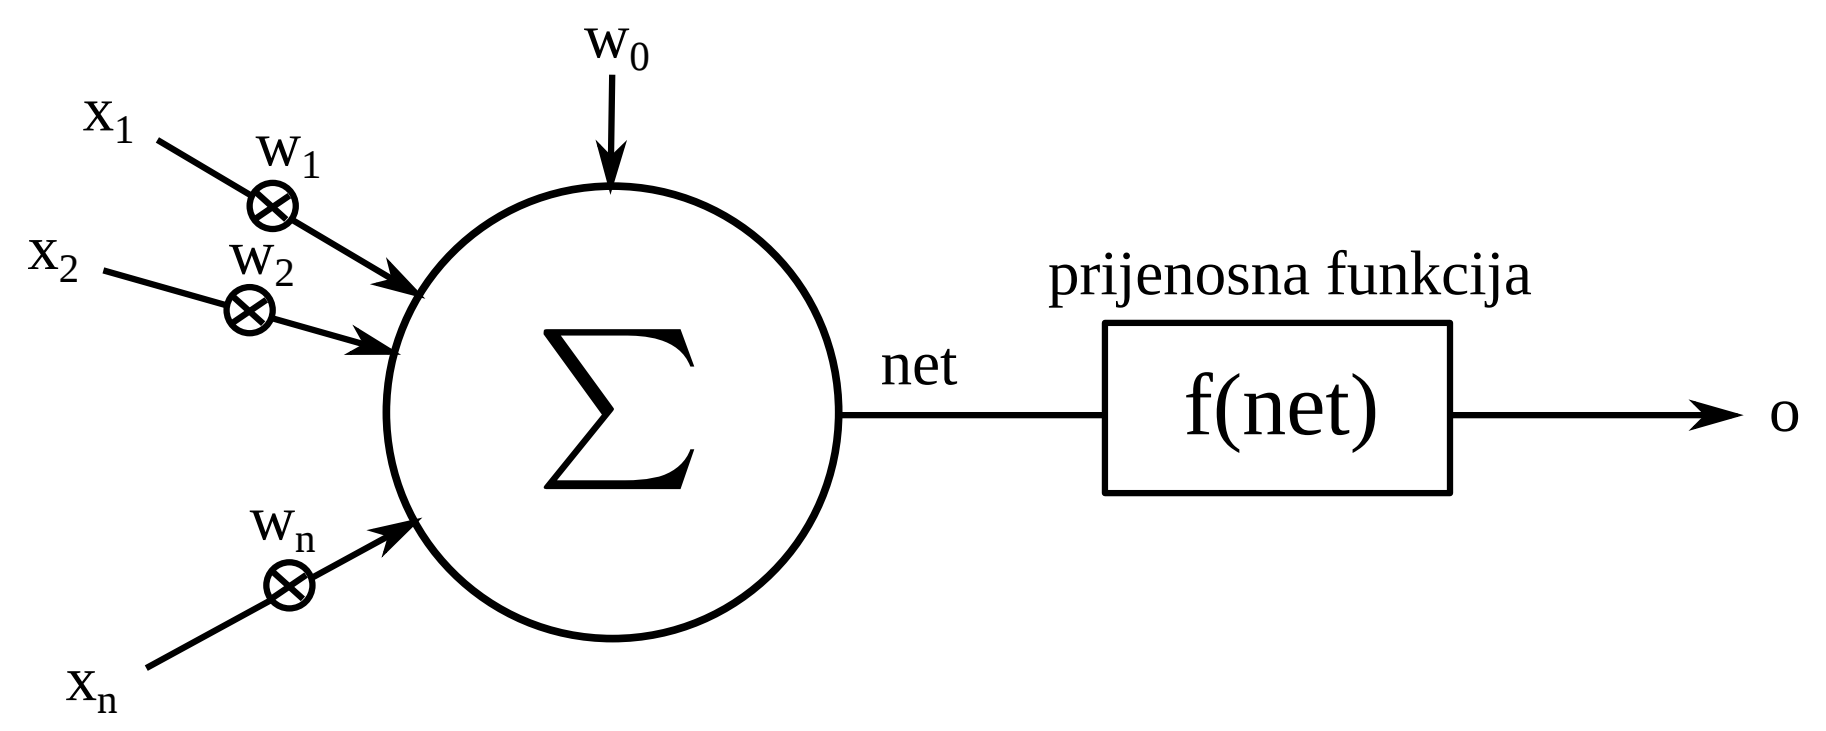
\includegraphics[width=\textwidth]{Extra/modelUmjetnogNeurona.png} 
		\caption{Model umjetnog neurona}
		\label{modelUmjetnogNeurona}
	\end{figure}
	
	Umjetni neuroni se povezuju u paralelne strukture različitih arhitektura koje omogućuju paralelnu obradu podataka \cite{skriptaNeuronskeMreze}. Arhitektura umjetne neuronske mreže opisuje kako su povezani umjetni neuroni u mreži i koliko ih ima. Postoje razne arhitekture neuronskih mreža, što jednostavnih, što kompleksnih, a svaka ima svoje prednosti i područja u kojima ima primjenu.
	
	Umjetni neuroni se u umjetnim neuronskim mrežama često organiziraju u slojeve. Tako razlikujemo ulazni sloj, skrivene slojeve i izlazni sloj. Skriveni slojevi i izlazni sloj se sastoje od umjetnih neurona dok ulazni sloj zapravo ne sadrži umjetne neurone kakvi su opisani u odjeljku iznad. Neuroni ulaznog sloja na svoje ulaze samo primaju ulazne podatke neuronske mreže te ih dalje prosljeđuju neuronima prvog skrivenog sloja.
	
	Umjetne neuronske mreže danas imaju vrlo široku primjenu, od obrade slika i signala, prepoznavanja uzoraka, kompresije slika, upravljanja, financija... \cite{skriptaNeuronskeMreze}. Glavne prednosti neuronskih mreža su vrlo dobra sposobnost generalizacije i učenja, čak i uz neprecizne ulazne podatke.Njihova glavna mana je nemogućnost interpretacije njihovog ponašanja, iako su računalni znanstvenici počeli razvijati metode za dedukciju strategija koje neuronske mreže nauče \cite{MITNeuralNet}. Znanje koje neuronske mreže nauče iz podataka je implicitno pohranjeno u način povezivanja neurone i težine veza između njih \cite{skriptaNeuronskeMreze}. Stoga je teško razumjeti zašto je neuronska mreža za neki ulaz dala baš taj izraz. Također, teško je prepoznati kakvu konkretnu ulogu u sveukupnoj obradi ulaza ima pojedini neuron u mreži.
	
	\section{Elmanova neuronska mreža}
	\label{pog:ElmanovaMreza}
	
		Elmanova neuronska mreža je jednostavna povratna neuronska mreža (\textit{eng. Recurrent Neural Network}). Glavna karakteristika takvih mreža je da imaju neku vrstu povratne veze ili vremenski odgođene veze \cite{ElmanNetSite}.
		
		Elmanova neuronska mreža se sastoji od ulaznog sloja, jednog skrivenog sloja i izlaznog sloja. Skriveni sloj ove mreže ima dodatan skriveni kontekst. Kontekst čine neuroni koji služe za pohranu kontekstnih podataka. Dodatno postoje veze iz izlaza skrivenog sloja prema kontekstu i veze iz konteksta prema ulazu u skriveni sloj. Izlaz iz skrivenog sloja se preko tih veza sprema u kontekst. Kod obrade sljedećeg ulaza u neuronsku mrežu skrivenom se sloju na ulaz dodatno stavljaju vrijednosti iz konteksta preko pripadajućih veza te se ukupan ulaz mreže i konteksta dalje obrađuje \cite{Elman}. Jednostavna shema Elmanove mreže prikazana je na slici \ref{ElmanovaMreza}.
		
		\begin{figure}[htb]
			\centering
			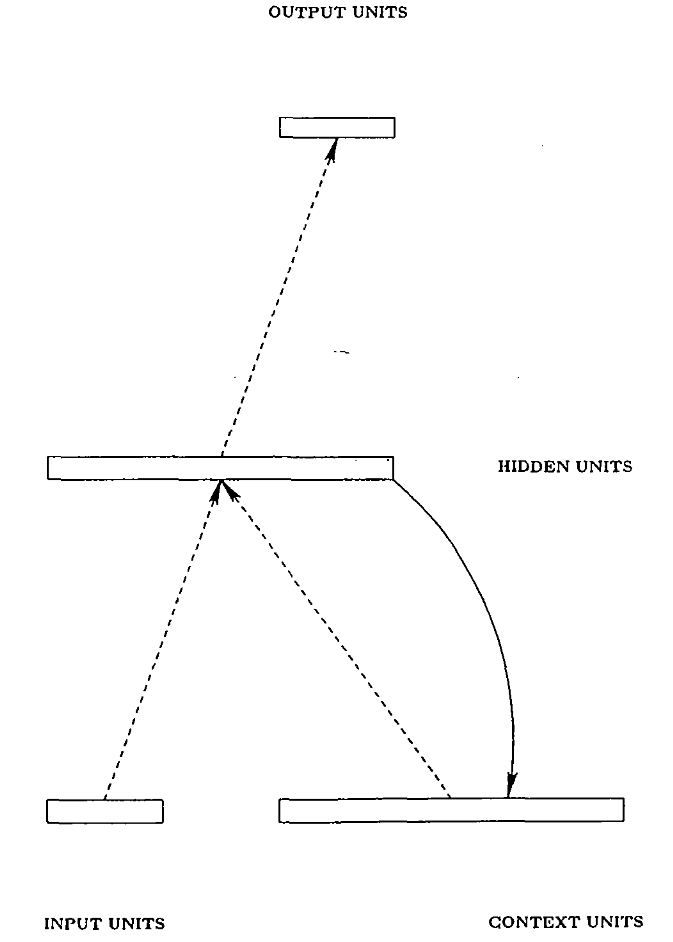
\includegraphics[width=0.9\textwidth]{Extra/ElmanovaMreza.png} 
			\caption{Shema Elmanove mreže \\
					 Napomena: iscrtkane linije označuju veze koje se mogu trenirati}
			\label{ElmanovaMreza}
		\end{figure}
		
		Ovime se omogućava da Elmanova mreža može pamtiti prošla stanja. Na ovaj način prijašnji ulazi u neuronsku mrežu utječu na rezultat obrade nekog budućeg ulaza.
		
		Ovo je korisno svojstvo za model inteligentnog igrača Zatvorenikove dileme, s obzirom da je prirodno da prijašnje interakcije sa drugim igračem utječu na nove odluke.
	
\chapter{Evolucijsko računanje}
\label{pog:EvolucijskoRacunanje}

	Evolucijsko računanje je grana umjetne inteligencije koja se najčešće bavi rješavanjem optimizacijskih problema. Začeci ove grane sežu još u kasne 50-te godine prošlog stoljeća. Evolucijsko računanje se može podijeliti u tri grane \cite{skriptaEvolucijskoRacunarstvo}: 
	\begin{itemize}
		\item \textit{evolucijske algoritme}
		\item \textit{algoritme rojeva}
		\item \textit{ostale algoritme}
	\end{itemize}
	
	Neki od algoritama iz grane evolucijskih algoritama su evolucijske strategije, evolucijsko programiranje, genetski algoritam i genetsko programiranje \cite{skriptaEvolucijskoRacunarstvo}.
	
	U grani algoritma rojeva nalaze se mravlji algoritmi, algoritam roja čestica, algoritmi pčela i drugi \cite{skriptaEvolucijskoRacunarstvo}.
	
	Neki do značajnih algoritama iz grane ostali algoritmi pripadaju umjetni imunološki algoritmi, algoritam diferencijske evolucije i algoritam harmonijske pretrage \cite{skriptaEvolucijskoRacunarstvo}.
	
	Područje evolucijskog računanja također pripada području metaheuristika. Metaheuristika je skup algoritamskih koncepata koji se koriste za definiranje heurističkih metoda primjenjivih na široki skup problema \cite{skriptaEvolucijskoRacunarstvo}. Heurističke metode su algoritmi koji pronalaze rješenja problema koja su zadovoljavajuće dobra, ali ne nužno optimalna. Heurističke metode obično imaju relativnu nisku računsku složenost \cite{skriptaEvolucijskoRacunarstvo}.

	\section{Optimizacija}
	\label{pog:Optimizacija}
	
		Kao što je ranije navedeno, algoritmi iz područja evolucijskog računanja se često koriste u problemima optimizacije. Optimizaciju možemo definirati kao postupak pronalaženja najboljeg rješenja problema. Uz svako rješenje se pridružuje funkcija dobrote ili funkcija kazne. Ako se rješenjima pridružuje funkcija dobrote, optimizacijski postupak će tražiti rješenje tako da pokuša maksimizirati funkciju dobrote. Ako se pak rješenjima pridružuje funkcija kazne, optimizacijski postupak će pokušati minimizirati funkciju kazne.\cite{skriptaEvolucijskoRacunarstvo}

		Bitno je reći da kada gledamo optimizacijske algoritme iz područja evolucijskog računanja, niti jedan od njih se ne može istaknuti kao generalno najbolji algoritam. Svaki od tih algoritama je dobar u određenim primjenama, dok u drugim primjenama drugi optimizacijski algoritmi daju bolje rezultate. U prosjeku nema značajnih razlika u globalnim performansama kada se gleda prosjek po svim mogućim funkcijama cijene.\cite{skriptaEvolucijskoRacunarstvo}
	
	\section{Genetski algoritam}
	\label{pog:Genetski algoritam}
	
		Genetski algoritam je algoritam iz grane evolucijskih algoritama. Općenito, svi pristupi iz grane evolucijskih algoritama crpe inspiraciju iz Darwinove teorije o postanku vrsta, koja se temelji na pet pretpostavki \cite{skriptaEvolucijskoRacunarstvo}:
		\begin{enumerate}
			\item potomaka uvijek ima više nego je potrebno
			\item veličina populacije je približno stalna u vremenu
			\item hrana je ograničen resurs
			\item ne postoje dvije potpuno identične jedinke kod vrsta koje se seksualno razmnožavaju - postoje varijacije
			\item većina varijacija se prenosi nasljeđem
		\end{enumerate}
		
		Genetski algoritam je jedan od algoritama koji rješavaju optimizacijske probleme, a koji izravno utjelovljuje navedene postavke. Genetski algoritam zapravo nije jedinstven, već se može implementirati na različite načine. \cite{skriptaEvolucijskoRacunarstvo}
		
		Ideja genetskog algoritma je modeliranje evolucijskog procesa. U algoritmu postoji populacija jedinki, koje zapravo predstavljaju neka od mogućih rješenja problema. Cilj algoritma je kroz selekciju roditelja, stvaranje novih jedinki korištenjem operatora križanja nad roditeljima i korištenje operatora mutiranja nad novim jedinkama. Selekcija roditelja bi trebala ovisiti o nekakvoj metrici uspješnosti - uspješniji roditelji bi trebali imati veće izglede da budu odabrani za križanje. Ta metrika se obično naziva dobrota. Takvim postupkom se očekuje da će se kontinuiranim križanjem uspješnih roditelja i mutiranjem njihove djece stvarati bolja rješenja. Ovo je zapravo svojevrstan ekvivalent prirodnoj selekciji, to jest preživljavanju najboljih.
	
		Varijacije u implementaciji se mogu pojavljivati u načinu mutiranja, križanja, selekcije, ali i magnitudi izmjena u populaciji u jednoj iteraciji algoritma. 
		
		Tako u jednoj krajnosti imamo takozvani \textit{eliminacijski genetski algoritam} u kojem se u jednoj iteraciji samo jedna jedinka zamjenjuje jednim novonastalim djetetom. Novo dijete već u sljedećem koraku može biti roditelj.
		
		U drugoj krajnosti imamo \textit{generacijski genetski algoritam}. U njemu se u jednoj iteraciji iz jedne populacije biraju roditelji čija se djeca spremaju u novu populaciju sve dok nova populacije ne dosegne veličinu populacije roditelja. Tada populacija djece zamjenjuje populaciju roditelja. U ovoj varijanti dijete može biti roditelj tek kada populacija djece postane populacija roditelja, to jest u sljedećoj iteraciji. \cite{skriptaEvolucijskoRacunarstvo}
		
		Operator križanja se primjenjuje nad dvije jedinke (roditelji) i iz njih stvara dijete. Može se implementirati na razne načine, ali generalno ovaj operator često vrši kontrakciju nad populacijom. To znači da se primjenom ovog operatora obično gubi raznolikost između jedinki te one u prosjeku postaju sve sličnije. \cite{skriptaEvolucijskoRacunarstvo}
		
		Operator mutacije ima upravo suprotno svojstvo. On vrši nasumične izmjene nad jedinkama i time im vraća raznolikost. Njegova važna uloga je izbaciti populaciju iz lokalnih maksimuma u prostoru rješenja \cite{skriptaEvolucijskoRacunarstvo}.
	
\chapter{Implementacija inteligentnog igrača}
\label{pog:Implementacija}

	Inteligentni igrač Zatvorenikove dileme modeliran je jednostavnom Elmanovom neuronskom mrežom. Mreža se sastoji od ulaznog sloja, jednog skrivenog sloja sa kontekstom i izlaznog sloja. Svi slojevi su potpuno povezani. Veze između izlaza skrivenog sloja i konteksta su jedan-na-jedan, to jest izlaz jednog neurona se preslikava u "kopiju" tog neurona u kontekstu. To implicitno znači da skriveni kontekst ima jednak broj neurona kao i sam skriveni sloj. Veze između konteksta i ulaza u neurone skrivenog sloja su svaki-sa-svakim, isto kao i između ostalih slojeva u mreži.
	
	Korištena mreža je arhitekture 1 x 8 x 1. Ulaz u mrežu je brojčana vrijednost odluke suparničkog igrača iz prijašnje runde. Ako prijašnje runde još nije bilo, tada se na ulaz dovodi 0. Odluka o suradnji je brojčano kodirana vrijednošću 1, a odluka o izdaju vrijednošću -1. Izlaz mreže je brojčana vrijednost odluke koju će inteligentni igrač odigrati u ovoj rundi Zatvorenikove dileme.

	\section{Učenje inteligentnog igrača}
	\label{pog:Ucenje}
	
	S obzirom na karakteristike Zatvorenikove dileme i dinamiku okruženja u kojem inteligentni igrač mora donositi odluke,često korišteno nadzirano učenje neuronske mreže algoritmom propagacije unazad ovdje nije praktično.
	
	Ako bismo koristili algoritam propagacije unazad, morali bismo za svaki ulaz definirati očekivani (najbolji) izlaz, to jest optimalnu odluku u toj situaciji. S obzirom da u ovom problemu postoje samo 3 moguća ulaza u mrežu (0 ako se radi o prvoj rundi, 1 ako je u prijašnjoj rundi suparnički igrač surađivao i -1 ako je izdao ovog igrača), skup za učenje bi bio premalen. Također, problem u tom pristupu je to što bismo time inteligentnom igraču zapravo predstavljali problem Zatvorenikove dileme sa samo jednom iteracijom, a taj problem ima potpuno različit pristup u odnosu na iterirajuću Zatvorenikovu dilemu, kao što je prije raspravljeno. Još jedan problem je u tome što je zapravo teško odrediti što je najbolji potez koji igrač može odigrati u nekom okruženju. 
	
	Bolji pristup je zato neka vrsta podržanog učenja. Općenito se kod podržanog učenja razmatra interakcija agenta i njegove okoline. Agent dobiva informacije iz okolina i na temelju njih vrši akcije. Za izvršene akcije agent dobiva nagrade ili kazne. Cilj podržanog učenja je razviti strategiju ponašanja agenta koja će maksimizirati njegovu nagradu. \textit{\textbf{???}}
	
	Zbog toga je za ovaj problem odlučeno koristiti jednu drugu tehniku, a to je učenje neuronske mreže genetskim algoritmom. Ideja ove tehnike je koristiti genetski algoritam kao algoritam optimizacije nad neuronskim mrežama. Cilj optimizacije je pronaći težine veza između neurona (i pomake svakog neurona) koje će davati najbolje (ili barem dovoljno dobre) performanse neuronske mreže u igri Zatvorenikove dileme.
	
	\subsection{Parametri genetskog algoritma}
	\label{pog:ParametriGenetskogAlg}
	
		Za genetski algoritam nad neuronskom mrežom je samo potrebno definirati kriterij i postupak nagrađivanja te rangiranja neuronskih mreža, način selekcije roditelja, operatore križanja i mutacije sa njihovim parametrima, magnitudu izmjena u populaciji, veličinu populacije i kriterij za završetak algoritma.
		
		Kao kriterij nagrađivanja i rangiranja neuronskih mreža iz populacije koriste se bodovi dobiveni igranjem Zatvorenikove dileme. Svaka mreža iz populacije igra zadani broj rundi Zatvorenikove dileme sa svakom drugom neuronskom mrežom i sa samom sobom. Broj rundi koje će dvije mreže međusobno odigrati može podešavati sam korisnik. Dobiveni bodovi se zbrajaju te dobivena suma predstavlja takozvanu dobrotu neuronske mreže. Ti bodovi se računaju svaki puta nakon stvaranja nove generacije neuronskih mreža. Ovaj način nagrađivanja savršeno odgovara za problem iterirajuće Zatvorenikove dileme jer ovime nije nužno da neuronska mreža mora pobjeđivati druge neuronske mreže u direktnom okršaju, već je bitno da kontinuirano može dobivati dosta bodova protiv neuronskih mreža sa raznim strategijama.
		
		Za selekciju roditelja je korištena proporcionalan selekcija - vjerojatnost da će neuronska mreža biti odabrana za roditelja je proporcionalna njezinim relativnim bodovima u odnosu na druge. Programsko rješenje također omogućava da korisnik odredi hoće li se dijete stvarati iz jednog ili dva roditelja. Ako je odabrano da dijete nastaje samo iz jednog roditelja, tada dijete nastaje kao kopija roditelja te se zatim nad njim primjenjuje operator mutacije. Dakle, u tom se slučaju ne koristi operator križanja.
		
		Kod operatora križanja se za određivanje parametara\footnote{Za parametre neuronske mreže podrazumijevaju se težine veza između neurona i pomaci (eng. \textit{biases})} djeteta nasumično biraju ekvivalentni parametri jednog od roditelja. Odabir roditelja od kojeg će se naslijediti konkretan parametar se ponovno vrši proporcionalnom selekcijom. Dakle, za svaki parametar vrijedi da je vjerojatnost da će on biti naslijeđen od nekog roditelja je proporcionalna relativnoj dobroti tog roditelja u odnosu na drugog roditelja.
		
		Operator mutacije se koristi dvjema vrstama mutacija - velikim i malim. Male mutacije su češće i manjeg intenziteta, dok su velike rjeđe i većeg intenziteta. Nakon stvaranja novog djeteta, svaki parametar ima vjerojatnost da će nad njim biti izvršen operator male mutacije. Ako ne dođe do male mutacije, parametar ima vjerojatnost da se nad njim izvrši velika mutacija. Mutacija funkcionira tako da se generira slučajan broj u nekom intervalu te se dobiveni broj pribraja vrijednosti parametra. Kod velike mutacije taj je interval širi. Interval je uvijek definiran oko nule. Vjerojatnosti i magnitude velike te male mutacije korisnik može sam određivati.
		
		Korišten je \textit{generacijski genetski algoritam}. Dakle, u jednoj iteraciji se cijela populacija jedinki zamjenjuje. Iznimka je jedino da se najbolja mreža iz prošle generacije direktno kopira u novu generaciju bez izmjena. Time se nastoji očuvati svojstvo elitizma \footnote{Elitizam je svojstvo algoritma da ne može izgubi najbolje pronađeno rješenje \cite{skriptaEvolucijskoRacunarstvo}}. 
	
		Ostale parametri genetskog algoritma su: veličina populacije i maksimalni dopušteni broj generiranih populacija prije završetka algoritma. Te parametre korisnik može sam podešavati.
	
\chapter{Definiranje pokusa}
\label{pog:Pokus}

	Pokus je zamišljen tako da se 20 puta pokrene treniranje neuronskim mreža. Na kraju svakog treniranja se izvlači najbolja neuronska mreža iz zadnje generacije te se sa njom igra Zatvorenikova dilema sa ciljem da se utvrdi postojanje određenih svojstava u strategiji igranja te neuronske mreže. Svojstva koja će se ispitivati su:
	\begin{itemize}
		\item Ljubaznost (eng. \textit{niceness})
		\item sklonost opraštanju (eng. \textit{forgiveness})
		\item provokabilnost (eng. \textit{provocability})
	\end{itemize}
	
	Navedena svojstva su opisana ranije u poglavlju \ref{pog:ZatvorenikovaDilema}. Promatrat će se učestalost pojavljivanja pojedinog svojstva u strategijama najboljih igrača. Iz toga će se pokušati izvesti zaključak o tome jesu li i koliko navedena svojstva robusna i poželjna u generalnoj Zatvorenikovoj dilemi neovisnoj o drugim igračima.
	
	

% \Blindtext


%-------------------------------------------------------------------------------
\chapter{Rezultati i rasprava}
\label{pog:rezultati_i_rasprava}

	\begin{longtblr}[
		caption={Rezultati pokusa},
		label=Results,
		entry=none
		]{
			width = \textwidth,
			colspec={|X[1,l]|X[1.6, l]|X[3, l]|X[3,l]|X[1.2,l]|}, 
			rowhead = 0,
		} %definicija širine tablice, širine stupaca, poravnanje i broja redaka naslova tablice
		\hline 
		\textbf{Redni\\broj\\pokusa} & \textbf{Ljubaznost} & \textbf{Opraštanje} & \textbf{Provokabilnost} & \textbf{Najbolji\\rezultat} \\ \hline
		\textbf{1} & da & do 3 uzastopne izdaje & 1 izdaja nakon 3 uzastopne izdaje, nakon toga se resetira & 70:15 \\ \hline
		\textbf{2} & ne & ne oprašta & stalno izdaje & 16:16 \\ \hline
		\textbf{3} & ne & ne oprašta & stalno izdaje & 16:16 \\ \hline
		\textbf{4} & ne & oprašta gotovo uvijek & rijetko izdaje ako je izdana & 80:0 \\ \hline
		\textbf{5} & ne &ne oprašta & stalno izdaje & 16:16 \\ \hline
		\textbf{6} & da & oprašta sve & nikada ne izdaje & 80:0 \\ \hline
		\textbf{7} & da & oprašta sve & nikada ne izdaje & 80:0 \\ \hline
		\textbf{8} & - & - & - & - \\ \hline
		\textbf{9} & - & - & - & - \\ \hline
		\textbf{10} & - & - & - & - \\ \hline
		\textbf{11} & - & - & - & - \\ \hline
		\textbf{12} & - & - & - & - \\ \hline
		\textbf{13} & - & - & - & - \\ \hline
		\textbf{14} & - & - & - & - \\ \hline
		\textbf{15} & - & - & - & - \\ \hline
		\textbf{16} & - & - & - & - \\ \hline
		\textbf{17} & - & - & - & - \\ \hline
		\textbf{18} & - & - & - & - \\ \hline
		\textbf{19} & - & - & - & - \\ \hline
		\textbf{20} & - & - & - & - \\ \hline
	\end{longtblr}
	
	Napomene: Igrač iz 4. pokusa je pokoran - ako je dovoljno puta izdan, počinje samo surađivati i dopuštati da ga se iskorištava. Međutim, ako ga drugi igrač ne izdaje, on će pokušati izdati njega u prosjeku svaki drugi puta. 

	\section{Rasprava}


% \Blindtext


%--- ZAKLJUČAK / CONCLUSION ----------------------------------------------------
\chapter{Zaključak}
\label{pog:zakljucak}

Na kraju rada piše se kratak zaključak, duljine do najviše jedne stranice. 
% \blindtext


%--- LITERATURA / REFERENCES ---------------------------------------------------

% Literatura se automatski generira iz zadane .bib datoteke / References are automatically generated from the supplied .bib file
% Upiši ime BibTeX datoteke bez .bib nastavka / Enter the name of the BibTeX file without .bib extension
\bibliography{literatura}



%--- SAŽETAK / ABSTRACT --------------------------------------------------------

% Sažetak na hrvatskom
\begin{sazetak}
	
	Zatvorenikova dilema je poznati problem iz područja teorije igara. U jezgri dileme je sukob između racionalnog razmišljanja maksimiziranja vlastite dobiti dvaju igrača koje ih dovodi do sub-optimalne pozicija te međusobne suradnje koja je korisna za oba igrača. Ovaj rad se bavi problemom izrade inteligentnog igrača koji će moći igrati iterirajući problem Zatvorenikove dileme. Za modeliranje inteligentnog igrača korištena je Elmanova neuronska mreža. Mreža je trenirana generacijskim genetskim algoritmom. Pokusom je pokušano utvrditi učestalost pojedinih karakteristika strategije igranja inteligentnog igrača. Time se želi utvrditi robusnost strategija igranja Zatvorenikove dileme koje posjeduju tražene karakteristike. Karakteristike koje se promatraju su: ljubaznost, sklonost opraštanju i provokabilnost.

  % \blindtext
\end{sazetak}

\begin{kljucnerijeci}
	Zatvorenikova dilema, umjetna inteligencija, umjetne neuronske mreže, inteligentni igrač, Elmanova neuronska mreža
\end{kljucnerijeci}


% Abstract in English
\begin{abstract}
	
	Prisoner's Dilemma is famous problem in game theory. The core of the Dilemma is the conflict between rational thinking of maximizing personal gain that brings two players in sub-optimal position and mutual cooperation that brings benefits for both players. This thesis has goal to create intelligent player for iterated Prisoner's Dilemma. For modelling an intelligent player was used Elman's neural network. The network was trained with generational genetic algorithm. Experiment was used to determine frequency of specific characteristics in the strategies used by the intelligent player. Goal of the experiment is to show how robust strategies that have specified characteristics are. Characteristics that were observed are: niceness, forgiveness and provocability.
	
  % \blindtext 
\end{abstract}

\begin{keywords}
  Prisoner's dilemma, Artificial intelligence, Artificial neural networks, Intelligent player, Elman's neural network
\end{keywords}


%--- PRIVITCI / APPENDIX -------------------------------------------------------

% Sva poglavlja koja slijede će biti označena slovom i riječi privitak / All following chapters will be denoted with an appendix and a letter
\backmatter

\chapter{Programski kod}

	U sklopu ovog završnog rada izrađena je jednostavna aplikacija u programskom jeziku \textit{Java}. Aplikacija omogućuje treniranje Elmanove neuronske mreže genetske mreže i igranje Zatvorenikove dileme.
	
	Aplikacija u početnom prozoru prikazuje 4 gumba pomoći kojih nudi sljedeće mogućnosti:
	\begin{itemize}
		\item Treniranje neuronske mreže
		\item Igranje Zatvorenikove dileme
		\item Učitavanje postojeće neuronske mreže
		\item Prikaz kratkog opisa aplikacije u odvojenom prozoru.
	\end{itemize}
	
	Kod izbora treniranja neuronske mreže prikazuje se prozor u kojem se mogu podesiti slijedeći parametri genetskog algoritma:
	\begin{itemize}
		\item Vjerojatnost male mutacije
		\item Magnituda male mutacije
		\item Vjerojatnost velike mutacije (kada se ne realizira mala mutacija)
		\item Magnituda velike mutacije
		\item Broj roditelja (1 ili 2)
		\item Veličina populacije
		\item Najveći broj generiranih generacija prije završavanja algoritma
		\item Broj iteracija u jednoj igri Zatvorenikove dileme prilikom određivanja dobrote svake mreže
	\end{itemize}
	
	Nakon podešavanja parametara pokreće se genetski algoritam. Program je podešen tako da sprema najbolju, medijalnu i najlošiju neuronsku mrežu svake pete generacije u direktorij \textit{src/main/resources} Maven projekta. Na dnu prozora je prikazan teoretski najveća moguća dobrota koju neka mreža može ostvariti. Dodatno, za svaku se generaciju ispisuju slijedeći podaci:
	\begin{itemize}
		\item Dobrota najbolje mreže iz te generacije
		\item Dobrota medijalne mreže iz te generacije
		\item Dobrota najlošije mreže iz te generacije
	\end{itemize}
	
	Po završetku genetskog algoritma omogućeno je da korisnik igra Zatvorenikovu dilemu protiv najbolje mreže iz posljednje generacije genetskog algoritma. Igra se sastoji od 16 rundi Zatvorenikove dileme. Prozor prikazuje ostvarene bodove svakog igrača u svakoj rundi te ukupno ostvarene bodove. Neuronska mreža uvijek igra kao \textit{Player 2}, dok je korisnik \textit{Player 1}.
	
	Kod izbora igranja Zatvorenikove dileme priprema se Zatvorenikova dilema za dva korisnička igrača. Prvo se prikazuje prozor koji prikazuje kontrole za oba igrača. kontrole za svakog igrača su prikazane u tablici \ref{kontrole} i stalno su iste.
	
	\begin{longtblr}[
		caption={Kontrole pojedinog igrača},
		label=kontrole,
		entry=none
		]{
			width = \textwidth,
			colspec={|X[1,l]|X[2, l]|X[2, l]|X[2,l]|}, 
			rowhead = 0,
		} %definicija širine tablice, širine stupaca, poravnanje i broja redaka naslova tablice
		\hline 
		 & Suradnja & Izdaja \\ \hline
		\textit{Player 1} & W & S \\ \hline
		\textit{Player 2} & P & L \\ \hline
	\end{longtblr}
	
	Nakon toga se prikazuje prozor koji prikazuje osvojene bodove svakog igrača na identičan način kao i prilikom igranja Zatvorenikove dileme sa inteligentnim igračem nakon provođenja genetskog algoritma. Igra se ponovno sastoji od 16 rundi.
	
	Kod odabira učitavanja neuronske mreže iz datoteke otvara se prozor za odabir datoteke. Nakon što korisnik odabere datoteku aplikacija će pokušati učitati neuronski mrežu iz datoteke. Po završetku uspješnog učitavanja mreže pokreće se igra identično kao i nakon treniranja neuronske mreže genetičkim algoritmom.
	
	Za programsko rješenje korištena je \textit{Java 17}. Programski kod je organiziran kao Maven projekt. Dodatno je korištena vanjska Maven biblioteka \textit{nd4j-native-platform}. Korištena biblioteka nudi razne optimizirane operacije vezane uz linearnu algebru. Ono što je bilo bitno za ovaj projekt je bilo mogućnost optimiziranog matričnog množenja koje se koristi kod izračunavanja izlaza neuronske mreže. Za izradu grafičkog korisničkog sučelja (eng. \textit{GUI}) korištena je biblioteka \textit{Swing} koja je dio standardne biblioteke programskog jezika \textit{Java}.
	
	Izvorni kod programskog rješenja i sam završni rad dostupni su na javnom Git repozitoriju na \href{https://github.com/PetarBelosevic/Prisoner-s-Dilemma-AI.git}{poveznici}. Za korištenje programskog rješenja potrebno je preuzeti Git repozitorij, prevesti preuzeti Maven projekt (u naredbenom retku pomoću naredbe \textit{mvn compile}) i pokrenuti izvođenje iz razreda \textit{application.GUIApp} (u naredbenom retku pomoću naredbe \textit{mvn exec:java -Dexec.mainClass="application.GUIApp"}).
	
	U programskom kodu dostupno je nekoliko razreda koji nude slične funkcionalnosti kao i aplikacija sa grafičkim korisničkim sučeljem. Korišteni su za isprobavanje funkcionalnosti prije izrade grafičkog korisničkog sučelja.
	
	Prvi takav razred je \textit{game.application.ConsoleApp} koji omogućava igranje Zatvorenikove dileme koju igraju dva korisnika preko konzole. Kod oba igrača unos teksta "c" ili "C" se interpretira kao suradnja, a sve ostalo kao izdaja.
	
	Slijedeći takav razred je \textit{evolution.training.ConsoleTestingApp}. Razred omogućuje učitavanje neuronske mreže iz datoteke te igranje Zatvorenikove dileme protiv te mreže preko konzole.
	
	Posljednji takav razred je \textit{evolution.training.ConsoleTrainingApp}. Razred omogućava provođenje genetičkog algoritma kao i kod aplikacije sa grafičkim sučeljem. Postupak u konzoli ispisuje dobrote najbolje, medijalne i najlošije neuronske mreže svake 5-te generacije te iste neuronske mreže sprema u datoteke na disku.

% \Blindtext


\end{document}
